\documentclass{article}
\usepackage[utf8]{inputenc}
\usepackage[italian]{babel}
\usepackage{graphicx}
\title{Specifica e verifica di sistemi critici}
\author{Giulia}
\date{\today}

\begin{document}
\maketitle

\section{Abstract State Machines (parte 1): stato ASM}

Le ASM (Abstract State Machine) possono essere considerate FSM con stati generalizzati.
Rappresentano la forma matematica di macchine virtuali ed estendono la nozione di
Finite State Machine ampliando la definizione di stato e modificando la forma delle transizioni.

Si passa da stati di controllo non strutturati a \textbf{stati strutturati} che modellano:
\begin{itemize}
    \item dati complessi arbitrari (con domini di base e funzioni per la struttura);
    \item operazioni per la manipolazione di dati.
\end{itemize}

Lo stato è una struttura \emph{multi-sorted} (si possono avere domini di qualsiasi tipo)
\emph{first-order} (usa quantificatori), ovvero un'algebra del primo ordine.

Le transizioni sono \textbf{regole} che descrivono il cambiamento delle funzioni da uno
stato al successivo (regola di transizione base: \texttt{if Condition then Updates}).

I costruttori di regole sono diversi, ma finiti e semplici:
\begin{itemize}
    \item parallelismo (\texttt{par}) e azioni sequenziali (\texttt{seq});
    \item iterazioni (\texttt{while}) e invocazione di sottomacchine;
    \item non-determinismo (\texttt{choose}) e parallelismo sincrono non limitato (\texttt{forall});
    \item agenti multipli sincroni/asincroni.
\end{itemize}

Le ASM sono analoghe alle FSM; le differenze principali riguardano:
\begin{itemize}
    \item \textbf{la concezione degli stati}: nelle FSM esiste un unico stato di controllo
    (\emph{control state}), che può assumere valori in un insieme \emph{finito} di un certo
    tipo, mentre nelle ASM lo stato è più complesso (algebra);
    \item \textbf{le condizioni di input e le azioni di output}: nelle FSM si usa un alfabeto
    finito, mentre nelle ASM l'input può essere una qualsiasi espressione e le azioni sono generali.
\end{itemize}

Per riassumere: gli stati di una ASM sono delle strutture algebriche, dette (semplicemente) algebre. Le transizioni permettono di modificare la struttura algebrica durante la run o esecuzione della ASM

\subsection*{Vocabolario}

DEF. Un vocabolario (o segnatura) $\sum$ è una collezione finita di nomi di funzioni 
DEF. Fissato un vocabolario $\sum$, uno stato $A$ su $\sum$ è un 
insieme non vuoto $X$, detto superuniverso di $A$, con 
le interpretazioni dei nomi delle funzioni di $\sum$

\begin{itemize}
   \item se $f$ un nome di funzione n-aria (di n argomenti) di $\sum$ allora la sua interpretazione $f^A$ è una funzione di $X^n$ a $X$ 
   \item Se c è un nome di costante è un elemento di X di $\sum$, allora la sua interpretazione $C^A$ è un elemento di $X$
\end{itemize}

Le funzioni possono essere dinamiche o statiche, a seconda che l'iterpretazione del nome della funzione cambia o no da uno stato al sucessivo

\subsection*{Costanti}
Funzioni statiche costanti di arietà zero sono dette,  ogni vocabolario ASM contiene sempre le constanti statiche \textit{undef}, \textit{True}, \textit{False}. Altri esempi sono: i numeri sono costanti numeriche (l'utente può aggiurgerne di sue \texttt{minimoVoto = 18}

\subsection*{Funzioni statiche}
Le funzioni statiche (di arietà >0) sono definite tramite una legge fissa. Esempio di funzioni statiche sono le usuali operazioni tra numeri: +, -, ... tra booleni: AND, OR, ... Sono standard o l'utente ne può definire di sue es: \texttt{max(n, m)}

\subsection*{Funzioni dinamiche}
Cambiano la propria interpretazione al variare dello 
stato  Funzioni dinamiche di arietà zero sono le comuni variabili dei linguaggi di programmazione (Es: insertCoin, DisplayTime)

Esempio di stato ASM
Modello ASM: CLOCK real time
 Vocabolario (o segnatura) $\sum$
 \begin{itemize}
   \item Funzioni dinamiche: CurrTime: Real (viene incrementato dall’esterno), DisplayTime: Real
   \item Funzioni statiche: Delta: Real (intervallo di tempo) + : Real x Real -> Real (addizione)
\end{itemize}

\subsection*{Domini ASM}
Il superuniverso di uno stato ASM è “suddiviso” in universi, rappresentati dalle loro funzioni caratteristiche Se $X$ è il superuniverso dello stato $A$, l’ universo $G$ di $A$ è rappresentato dalla funzione $G: X \rightarrow Bool$ tale che $G(t) = true$ per tutti gli elementi $t$ del superuniverso $X$ di $A$ che 
formano la partizione (o sotto insieme) $G$; $G(t) = false,altrimenti$

Esempio: $X= {1,2,3, a,b, mario, pippo}$ ripartito in domini: 
$Interi={1,2,3}$, $Char={a,b}$, $String={mario, pippo}$

\subsection*{Termini ASM}
DEF.
I termini di $\sum$ sono espressioni sintattiche così costruite:
\begin{enumerate}
    \item Variabili $v_0$, $v_1$, $v_2$, ... sono termini
    \item  Costanti c of $\sum$ sono termini 
    \item Se f è un nome di funzione n-aria di $\sum$ e $t1, . . ., tn$ sono termini, allora $f(t1, . . . , tn)$ è un termine.
\end{enumerate}

Un termine che non contiene variabili è detto chiuso. Esempi: insertCoin, available(MILK), DisplayTime, …


\section{Abstract State Machines (parte 2): regole di transizione}
In matematica le algebre sono statiche : non cambiano col passare del tempo.

In Informatica, gli stati sono dinamici : evolvono essendo aggiornati durante le computazioni.

\textbf{Aggiornare stati astratti} (abstract states) significa cambiare l’interpretazione delle (o solo di alcune) funzioni dinamiche della segnatura della macchina.

Il modo in cui una macchina ASM aggiorna il proprio stato è descritto da regole di transizione (transitions rules) di una certa “forma".
L’insieme delle regole di transizione di una ASM definiscono la sintassi di un programma ASM
Sia $\sum$ un vocabolario. Le regole di transizione di una ASM sono espressioni sintattiche su $\sum$ generate come segue attraverso l’uso di costruttori di regole

\subsection*{Costruttore base: update rule}
Update Rule: \textbf{f (t1, . . . , tn) := s} dove $f$ è un nome di funzione dinamica n-aria di $\sum$ e $t_1, . . . , t_n$ e $s$ sono termini di $\sum$. Ossia nello stato successivo, il valore di $f$ per gli argomenti  $t_1, . . . , t_n$ è aggiornato a $s$. Se $f$ è 0-aria , cioè una variabile x, l’aggiornamento ha la forma \textbf{x := s}

L’update rule è il costrutto di base delle regole di transizione  e determina l’aggiornamento di una locazione ASM

\subsection*{Locazione ASM}

Nelle ASM gli stati sono associati a un insieme di valori di qualsiasi tipo,memorizzate in apposite locazioni. Matematicamente una locazione è definita come la coppia $(f, (v_1, ..., v_n))$ con $f$ nome di funzione e $(v_1, ..., v_n)$.

In uno stato S, una locazione ha un valore: l’interpretazione della funzione nello stato

Funzione può essere:  Variabili (0-arie)  x, y , ... e Funzioni (n-arie) f(1), name(2), ...

Le transizioni di stato delle ASM, tramite l’update rule, causano aggiornamenti dei valori contenuti nelle locazioni

Se $(loc = (f,(v_1, ..., v_n))$ ed valore $(loc) = a$, l’aggiornamento (o update) di loc ha la forma $f(v_1, ..., v_n) := newval$, l’aggiornamento cambia il valore di loc, e quindi di $f(v_1, ..., v_n)$, da a a newval

\subsection*{Costruttore if-then-else}
 Conditional Rule: \textbf{if} $\varphi$ \textbf{then} $R$ \textbf{else} $S$ ossia se $\varphi$ è vera, allora esegui R, altrimnti segui S 

 \subsection*{Classificazione delle funzioni ASM}
 Sia \textbf{M} una ASM e \textbf{env} l'ambiate di \textbf{M}

 \textbf{Dynamic:}  i valori dipendono dagli stati di \textbf{M}

 \begin{itemize}
     \item \textbf{in (monitored):} lette (non aggiornate) da M, scritte da env
      \item \textbf{out:} scritte (ma non lette) da M, lette da env
      \item \textbf{controlled:} lette e scritte da M
      \item \textbf{shared:} lette e scritte da M e da env 
 \end{itemize}

 \textbf{Derived:} valori computati da funzioni monitorate e funzioni statiche per mezzo di una “legge” o “schema” fissati a priori


\subsection*{Costruttori skip e let}
Skip Rule: non fare niente
Let Rule (se R ha parametri, realizza il passaggio per valore): let x = t in R(x) assegna il valore di t a x ed esegui R

\subsection*{Costruttore “par” per block rule}
Block Rule (composizione parallela): R e S sono eseguite in parallelo


 \textbf{par}

   \hspace{1cm} R

   \hspace{1cm} S

 \textbf{endpar}

\subsection*{Aggiornamenti Consistenti}
A causa del parallelismo (regole Block e Forall), una regola 
di transizione può richiedere più volte l’aggiornamento di una 
stessa funzione per gli stessi argomenti si richiede in tal caso che tali aggiornamenti siano 
consistenti (non posso aggiornare la stessa locazione conteporaneamente)

data la funzione $f(a1, …, an)$ in uno stato $S_i$ della macchina:
\begin{itemize}
  \item La coppia $loc=(f , (a1, . . . , an))$ è detta locazione e 
rappresenta matematicamente il valore di $f(a1, …, an)$ in 
memoria 
\item Un aggiornamento (o update) è la coppia:  $(loc,b) = ((f , (a1, . . . , an)), b)$ ossia l’interpretazione della funzione f in $S_i$ viene modificata per gli argomenti $a1, . . . , an$ con il valore $b$ in $S_{i+1}$
\item  Un update set è un insieme di aggiornamenti
\end{itemize}

DEF: Un update set U è consistente, se vale la condizione:
Per ogni locazione $(f , (a1, . . . , an))$,
se $((f , (a1, . . . , an)), b) \in U $  ed

$((f , (a1, . . . , an)), c)  \in U, allora b = c$

se b è diverso da c allora l'update si dice incosistente 

Se l’update set U è consistente, allora i suoi aggiornamenti 
possono essere effettivamente eseguiti (fired) in un dato stato.

Il risultato è un nuovo stato (di arrivo) dove le interpretazioni dei nomi delle funzioni dinamiche sono cambiati secondo U.

Le interpretazioni dei nomi delle funzioni statiche sono gli stessi
dello stato precedente (di partenza).

Le interpretazioni dei nomi delle funzioni monitorate sono date 
dall’ambiente esterno e possono dunque cambiare in maniera 
arbitraria.

\subsection*{Rule constructors}
(Macro) Call Rule: $r [t_1, . . . , t_n]$ ossia chiama r (regola con parametri) con argomenti t1, 
. . . , tn

Una definizione di regola per un nome di regola r di arietà n è 
un’espressione $r(x_1, ..., x_n) = R$ dove R è una regola di transizione.
In una call rule $r [t_1, . . . , t_n]$ le variabili $x_i$ che occorrono nel corpo R della definizione di r vengono sostituite dai parametri $t_i$(modularità: perché puoi definire la regola una volta e richiamarla più volte con argomenti diversi, senza riscriverla ogni volta)
Il risultato è che nel corpo RR
R ogni occorrenza di $x_i$ viene rimpiazzata da $t_i$: $R[x_1 \rightarrow t_1, x_2 \rightarrow t_2, ..., x_n \rightarrow t_n,]$

\subsection*{Costruttore seq}

Seq Rule (composizione sequenziale): \textbf{seq} R S \textbf{endseq} Significato: R e S sono eseguite in sequenza (gli update 
causati in R sono già visibili in S; lo stato tra R ed S non è 
visibile)



\subsection*{Costruttori  forall e choose}

Forall Rule: \textbf{forall} x \textbf{with} $\varphi$ \textbf{do} R[x] Significato: Esegui R in parallelo per ogni x che soddisfa $\varphi$ Implementa il concetto di parallelismo sincrono (potentially unbounded)

Choose Rule: \textbf{choose} x \textbf{with} $\varphi$ \textbf{do} R[x] Significato:  Esegui R per un x scelto random che soddisfi $\varphi$ Implementa il concetto di non-determinismo

\subsection*{ASMs: riassumendo. . .}

Una Abstract State Machine M è una terna:

\begin{itemize}
    \item un vocabolario $\sum$
    \item uno stati iniziale $A$ per $\sum$
    \item un insieme R di nomi di regole con un nome di regola di arietà zero, la cosidetta main rule (l’ “entry point” per l’esecuzione della macchina) e una definizione di regola per ogni nome di regola
\end{itemize}

La semantica delle regole di transizione è data dall’insieme di tutti gli aggiornamenti.

\subsection*{Eseguire una ASM}
La run(o esecuzione) di una ASM M è definita come Una sequenza finita o infinita S0, S1, …, Sn di stati di M, 
dove  S0 è lo stato iniziale e ciascun stato Sn+1 è ottenuto 
dal precedente Sn eseguendo simultaneamente
regole di transizione che sono eseguibili in Sn

\begin{figure}[h]
    \centering
    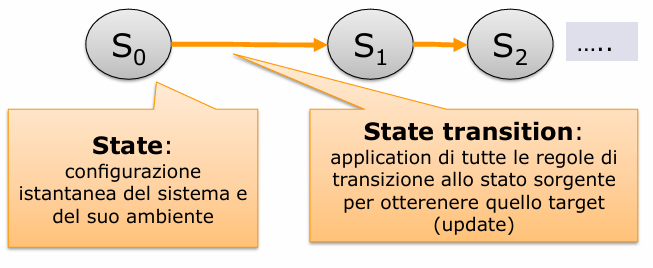
\includegraphics[width=0.6\textwidth]{immagini/stato.png}
\end{figure} 
n
b b
d n
\end{document}